%Copyright 2014 Jean-Philippe Eisenbarth
%This program is free software: you can 
%redistribute it and/or modify it under the terms of the GNU General Public 
%License as published by the Free Software Foundation, either version 3 of the 
%License, or (at your option) any later version.
%This program is distributed in the hope that it will be useful,but WITHOUT ANY 
%WARRANTY; without even the implied warranty of MERCHANTABILITY or FITNESS FOR A 
%PARTICULAR PURPOSE. See the GNU General Public License for more details.
%You should have received a copy of the GNU General Public License along with 
%this program.  If not, see <http://www.gnu.org/licenses/>.

%Based on the code of Yiannis Lazarides
%http://tex.stackexchange.com/questions/42602/software-requirements-specification-with-latex
%http://tex.stackexchange.com/users/963/yiannis-lazarides
%Also based on the template of Karl E. Wiegers
%http://www.se.rit.edu/~emad/teaching/slides/srs_template_sep14.pdf
%http://karlwiegers.com
\documentclass{scrreprt}
\usepackage{graphicx}
\usepackage{listings}
\usepackage{underscore}
\usepackage[bookmarks=true]{hyperref}
 
\usepackage[utf8]{inputenc}
\usepackage[english]{babel}
\usepackage{verbatim}
\usepackage{enumerate}
\hypersetup{
    bookmarks=false,    % show bookmarks bar?
    pdftitle={Software Requirement Specification},    % title
    pdfauthor={Kumbong Hermann,Akola Mbey Denis},                     % author
    pdfsubject={TeX and LaTeX},                        % subject of the document
    pdfkeywords={TeX, LaTeX, graphics, images}, % list of keywords
    colorlinks=true,       % false: boxed links; true: colored links
    linkcolor=blue,       % color of internal links
    citecolor=black,       % color of links to bibliography
    filecolor=black,        % color of file links
    urlcolor=purple,        % color of external links
    linktoc=page            % only page is linked
}%
\def\myversion{1.0 }
\date{}
%\title
\usepackage{hyperref}
\begin{document}

\begin{flushright}
    \rule{16cm}{5pt}\vskip1cm
    \begin{bfseries}
        \Huge{SOFTWARE REQUIREMENTS\\ SPECIFICATION}\\
        \vspace{1.9cm}
        for\\
        \vspace{1.9cm}
        Automatic Timetable Generator\\
        \vspace{1.9cm}
        \LARGE{Version \myversion approved}\\
        \vspace{1.9cm}
        %Prepared by Kumbong Hermann, Romeo Obeng and Adutwumah\\
        \vspace{1.9cm}
        Hex Group\\
        \vspace{1.9cm}
        \today\\
    \end{bfseries}
\end{flushright}

\tableofcontents


\chapter*{Revision History}

\begin{center}
    \begin{tabular}{|c|c|c|c|}
        \hline
	    Date & Author & Reason For Changes & Version\\
        \hline
	     18-03-2019& Kumbong Hermann N & First Draft & 1.0\\
        \hline
	   5-05-2019  &  Akola Mbey Denis & Second Draft &1.1 \\
        \hline
    \end{tabular}
\end{center}

\chapter{Introduction}

\section{Purpose}
The aim of this document is to delineate the software requirements specification for an automatic timetable generation software. The initial version of the software will be aimed at scheduling courses  at the university level and will serve as a course completion requirement for the COE 356 Software engineering course at KNUST. Future versions(not described in this document) will generalize the scheduling problem to cater for scheduling in non academic environments like hospitals, jobs etc.

\begin{comment}
$<$Identify the product whose software requirements are specified in this 
document, including the revision or release number. Describe the scope of the 
product that is covered by this SRS, particularly if this SRS describes only 
part of the system or a single subsystem.$>$
\end{comment}

\section{Document Conventions and Terminology}
This document follows MLA Format. Bold-faced text has been used to emphasize section
and sub-section headings. Highlighting is to point out words in the glossary and italicized text is
used to label and recognize diagrams. In addition the following jargon is used throughout the text:

\begin{center}
    \begin{tabular}{|c|p{10cm}|}
        \hline
	    Term & Meaning\\
        \hline
	     GUI&The graphical user interface is a form of user interface that allows users to interact with electronic devices through graphical icons and visual indicators such as secondary notation, instead of text-based user interfaces, typed command labels or text navigation. \\
        \hline
    \end{tabular}
\end{center}


\begin{comment}
$<$Describe any standards or typographical conventions that were followed when 
writing this SRS, such as fonts or highlighting that have special significance.  
For example, state whether priorities  for higher-level requirements are assumed 
to be inherited by detailed requirements, or whether every requirement statement 
is to have its own priority.$>$
\end{comment}

\section{Intended Audience and Reading Suggestions}
 The primary audience for this document consists of all group members of Hex(project manager, developers, section heads and analysts) together with the project supervisor. The information provided could also be of benefit to product users and the prospective users on whose suggestions this document heavily relies. The document includes but is not limited to: an overall description of the the project, a discussion on the interface requirements, an analysis of system features and a description of other non functional requirements of the system. The document follows the sequence just described and is meant to be followed in that order. However, a busy reader may omit the last section on non functional requirements. The section on external interface requirements is directed primarily at the front end department while the overall description of the project will most suit the needs of a prospective client or user. It is the duty of the project manager to peruse this document and to enforce its usage and distribution of tasks described.

\begin{comment}
$<$Describe the different types of reader that the document is intended for, 
such as developers, project managers, marketing staff, users, testers, and 
documentation writers. Describe what the rest of this SRS contains and how it is 
organized. Suggest a sequence for reading the document, beginning with the 
overview sections and proceeding through the sections that are most pertinent to 
each reader type.$>$
\end{comment}

\section{Project Scope}
 The  current goal of this project is to develop a software for automatically scheduling courses in the university milieu. Currently most universities use a manual or a semi manual system for generating timetables. Most software available works for high schools and primary schools and is not easily adapted to the university setting. The process which can last for even weeks necessitates a lot of effort in resolving clashes and adjusting the timetable to meet specific institutional needs or those of lectures and students. Our objectives in designing our own system to solve this problem are as follows:

\begin{itemize}
 \item Since at this moment we are unable to determine with certainty if the process can be completely automated, our goal is to automate the process of generating a timetable as much as possible providing the user of the system with little manual work to complete the timetable.
 \item  To reduce the effort and time that are currently expended in constructing a timetable by atleast 70 \%.
 \item To generate schedules that can 
 \item To design a system that can be customized to meet the specific scheduling needs of any institution.
 \item To develop a simple and intuitive user oriented system that requires as little user training as possible.
 \item To provide an solution for maintaining, publishing and sharing timetables to users.
\end{itemize} 
In order to achieve this,the software system must cover the following features and functions:
An \textbf{administrative} section which includes the following:
\begin{itemize}
\item Manage student profiles
\item manage lecturer's profiles
\item Manage the username,password,and change password.
\item Manage the add,or drop class
\item Manage the add,edit and delete class
\item Creation of Master Timetable
\item Accept changes to made by lecturers and students.
\end{itemize}
A \textbf{lecturer's} section which includes the following:
\begin{itemize}
\item View and print their own timetable
\item View and print the master timetable for one semester
\item Query on the class availability
\item Booking the class
\item Creation of the lecturer's timetable
\end{itemize}
A \textbf{Student} Section which includes the following:
\begin{itemize}
\item View and print the timetable for a semester
\item Change password
\item Creation of student's timetable
\item Request for change in timetable schedules
\end {itemize}



   
 
\begin{comment}
$<$Provide a short description of the software being specified and its purpose, 
including relevant benefits, objectives, and goals. Relate the software to 
corporate goals or business strategies. If a separate vision and scope document 
is available, refer to it rather than duplicating its contents here.$>$
\end{comment}
\section{References}
\begin{enumerate}
 \item IEEE. IEEE Std 830-1998 IEEE Recommended Practice for Software Requirements Specifications. IEEE Computer Society, 1998.
\end{enumerate}

\begin{comment}
$<$List any other documents or Web addresses to which this SRS refers. These may 
include user interface style guides, contracts, standards, system requirements 
specifications, use case documents, or a vision and scope document. Provide 
enough information so that the reader could access a copy of each reference, 
including title, author, version number, date, and source or location.$>$
\end{comment}


\chapter{Overall Description}

\section{Product Perspective}
  The Automatic Timetable Generation System is a closed source system comprising of 3  main components. The three components are as follows:
  
The Desktop platform is a stand alone program, which is a component of a larger timetable management system. The desktop component allows the user(administrator) to create and maintain a new timetable or to maintain a timetable already generated using the web component. This component is synchronized with the web app component which we describe next. The web app component provides a similar role to the desktop component. In addition to this it provides the means for managing user accounts. The mobile app component is meant for the end users of the timetable. (students, lecturers or other stakeholders). It provides them with a means of accessing their schedules and keeps them aware of any  updates. It also gives them the opportunity to request any changes in their schedules from the administrator.

\begin{comment}
$<$Describe the context and origin of the product being specified in this SRS.  
For example, state whether this product is a follow-on member of a product 
family, a replacement for certain existing systems, or a new, self-contained 
product. If the SRS defines a component of a larger system, relate the 
requirements of the larger system to the functionality of this software and 
identify interfaces between the two. A simple diagram that shows the major 
components of the overall system, subsystem interconnections, and external 
interfaces can be helpful.$>$
\end{comment}


\section{Product Functions}
The timetable management system alongside its subsystems shall perform the following features:

\begin{itemize}
 \item Provide the administrator with a means of creating a timetable template that satisfies the particular requirements(constraints) of his/her institution.
 \item Provide the administrator with a feature to automatically generate a timetable based on constraints they impose.
 \item Allow the administrator to apply manual changes to the timetable.
 \item \textbf{ When applying manual changes to the timetable, provide the administrator with real time alerts and information when constraints are not met.} (This feature is prime in importance)
 \item Provide the administrator on hints or information on available resources or solutions to resolving clashes.
 \item End users (students and lecturers) should have a module to provide the administrator with information required to generate schedules for them.
 \item End users (students and lecturers) should have a module to request changes in their schedules from the administrator.
 \item Provide the administrator or other stakeholders with an easy interface to import their data or to enter new data required for timetable generation and management.
 \item End users should have a module that informs them of their timetable and any changes that have been made to it. (This could be through the mobile or the web app component)
\end{itemize}

\begin{comment}
The main purpose purpose of this software product is to schedule and generate time tables within a few seconds to minutes. This will be relatively faster than the manual processes used to generate time tables which is a herculean task for management like the case of universities where a lot of courses have to be given <bf>time slots within the lecture hours of such institutions  without encountering collisions and ensuring each schedule meets the constraints of management. Some of which include the classroom size must be able to accommodate the number of students allocated to it. It is inappropriate to allocate a small classroom to a large group of students as it doesn't  effective teaching and learning.
Summarize the major functions the product must perform or must let the user 
perform. Details will be provided in Section 3, so only a high level summary 
(such as a bullet list) is needed here. Organize the functions to make them 
understandable to any reader of the SRS. A picture of the major groups of 
related requirements and how they relate, such as a top level data flow diagram 
or object class diagram, is often effective.$>$
\end{comment}
\section{User Classes and Characteristics}
The users of the system can be broadly classified into two major categories. Users can fall into only one category only or in both categories. However a user can only have one type of account. In a a case where a user can be in anyone category, they have to create an account for each new category. The categories are as follows:
\begin{enumerate}
\item \textbf{Administrators}\\
Administrators consist of anyone who are involved in the timetable generation process. More succinctly, administrators have the following privileges and roles:
 \begin{itemize}
 \item Can initiate the process of creating a new timetable.
 \item Has access to and can modify any timetable generated.
 \item Publishes the timetable and is responsible for responding to user requests and performing updates on the timetable.
 \item Fills the database with relevant information about resources such as (courses, lecturers, class size)
 \item Creates the atomic timetable template (for example is the timetable from monday to saturday or just weekdays, the number of working hours and all related information.)
 \item Decides on and implements scheduling and constraints and enforces that they are strictly followed.
 \item Assigns priorities to different users, tasks, resources.
 \end{itemize}
\item \textbf{End Users}
End users are the consumers of the timetable schedule. For instance a lecturer could have a schedule, a student may have a schedule, a particular class group have a schedule and so on. (Due to elective courses a student's schedule is not necessarily the same as that of their class. The discrepancy increases in a liberal art system). The end users have the following roles and privileges with respect to the system:
 \begin{itemize}
 \item Can view their personal schedules or those of any group they belong to.
 \item Can request changes to their schedules or that of any group they belong to(it is left to the administrator to decide whether or not to implement such changes.) 
 \end{itemize}
\end{enumerate}
\begin{comment}
$<$Identify the various user classes that you anticipate will use this product.  
User classes may be differentiated based on frequency of use, subset of product 
functions used, technical expertise, security or privilege levels, educational 
level, or experience. Describe the pertinent characteristics of each user class.  
Certain requirements may pertain only to certain user classes. Distinguish the 
most important user classes for this product from those who are less important 
to satisfy.$>$
\end{comment}
\section{Operating Environment}
  Our system is cross platform and does not dep
 on the hardware or architecture of the host system The web component is browser independent. In particular we support the particular operating systems.
  \begin{enumerate}
  \item \textbf{Mobile}\\
  \begin{enumerate}
  \item Android OS
  \item ios
  \end{enumerate}
  \item \textbf{Desktop}\\
  \begin{enumerate}
     \item Windows 7 and above
     \item Mac
     \item Linux
     \item Solaris
  \end{enumerate}
  \end{enumerate}
 
$<$Describe the environment in which the software will operate, including the 
hardware platform, operating system and versions, and any other software 
components or applications with which it must peacefully coexist.$>$
 
\section{Design and Implementation Constraints}
\textbf {Hardware requirements}
In order to develop a good  application  program, it is very important to choose the correct
hardware, software and technology. Below are some explanations of the hardware,
software and technology chosen as development tools for the Timetable Management
System 
\begin{itemize}
\item A processor of good processing speed $2.5MHz$ or more
\item 128MB DDR RAM ,256 MB is recommended
\item 10GB hard-disk space or higher
\item 56 Kbps Modem
\item Keyboard and mouse
\end {itemize}
\subsection {Programming / Scripting Language }
\begin {itemize}
\item \textbf{ Flask,a  Python Framework }
Python was created in 1991 by  Guido Van Rossum
 Flask is web development framework based on Python and it can  be
interspersed within Hypertext Markup Language (HTML), which makes developing
dynamic websites more accessible. Python Flask was selected to develop the Timetable Management System because it is a server side, cross-platform technology. Server-side actually refers to the fact that everything
Python Flask does occurs on the server instead of the client’s site. Its cross-platform means that
Python Flask runs on most operating systems, including Windows, UNIX, and Macintosh.  Besides that, when it comes to developing dynamic websites, Python Flask is better, faster and easier to learn than the alternatives. Of course, the main reason for
Python Flask being chosen to develop the website is it comes at no cost.It is open sourced.
\end {itemize}
\subsection {Web development tool}
\begin {itemize}
\item \textbf{Visual Studio Code,Atom,Sublime Text }
Visual Studio Code,Atom and Sublime Text were chosen as the text editors to develop the website as
well since the researcher is more familiar with using the text editors to develop a
websites
\end {itemize}
\subsection { Database and Technology}
 \begin{itemize}
\item \textbf{MySQL}
MySQL is a database management system (DBMS) for relational databases (therefore,
MySQL is an RDBMS), a database being a collection of interrelated data, be it text,
numbers, or binary files, that are stored and kept organized by the DBMS 
MySQL was selected to develop the database for this web based system because like Python Flask, MySQL offers excellent performance, portability and reliability, with moderate
learning curve at little to no cost because MySQL is the world’s most popular open
source database. Besides that, another reason for it being chosen is Python Flask  has good
support for MySQL.
\end{itemize}
 
\subsection{System Development }
The objective of the development phase is to convert the deliverables of the design
phase into a complete system. Most activities in the development phase addresses the
computer programs that make up the system, but this phase also puts in place the
hardware, software, and communications environment for the system and other
important elements of the overall system.
The activities in the development phase translate the system design produced in the
design phase into a working system. The development phase includes
activities for developing the system, testing the system, and to ensure the system
functions satisfy the functional process requirements. At the end of this phase, the
system will be ready for the activities of the testing phase. 
The Timetable Management System web base was developed after the system analysis
and system design phases. After gathering data from the system analysis stage and
designing the web base, the development is divided into three main sessions which a
\subsection{Database  Development}
The Timetable Management System used a relational database in its database
implementation because it can support multiple tables that store each item only once,
thus significantly reducing storage place. The database was created and using MySQL,
which is a GUI Client that works alongside MySQL Database server. 
\subsection{Testing}
The objective of this testing phase is to prove that the developed system (Timetable
Management System) satisfies the requirements defined earlier. Several types of tests
will be conducted in this phase. Testing is an important phase of system development
because it can ensure the system matches the specifications. Besides that, testing also
ensures that the system functions in the correct and proper manner with the minimum
amount of errors. 
\subsection {Unit Testing}
 Unit testing reveals syntax and semantic errors from the smallest programming unit. In
this thesis, unit testing is used to test each individual web page. Errors that are found in a
particular page of the website are thoroughly debugged and removed before starting to
develop another web page. Due to the dynamic nature of testing, there is no proper
testing documentation created. 
\subsection{Link or Integration Testing}
When each webpage of a particular Section in the Timetable Management System
passed the unit testing, integration test was carried out to ensure that pages are linked in
the correct flow and integrate properly into the entire website. Integration testing was
mainly conducted in “Administrator Module” Section “Lecturer Module” and “Student
Module” Section. All the buttons, hyperlinks and navigation bars were tested
 
\chapter{External Interface Requirements}

\section{User Interfaces}
The product presents to the user a friendly user interface. The GUI provides fields for the user to enter the data He/she wishes to schedule . In our case,the examinations officer can enter data comprising the classrooms,courses,and the names of the lecturers.

 

\section{Software Interfaces} 
\textbf{Developing end}
\begin{itemize}  
\item Python 3.6 -Python  is fast, secure, and reliable. 
\item MySQL server -Database connectivity and management\\
\textbf{Client End}\\
\item OS -Window 7 or higher -Very friendly and common OS
\item MySQL server -Database connectivity.
\end{itemize}

\section{Communications Interfaces}
\begin{itemize}
 \item NIC (Network Interface Card) - It is a computer hardware component that allows a computer to
connect to a network. NICs may be used for both wired and wireless connections.
\item CAT 5 network cable- for high signal integrity
\item  TCP/IP protocol- Internet service provider to access and share information over the
Internet
\item Ethernet Communications Interface- Ethernet is a frame-based computer network
technology for local area networks (LANs)
\item Ubiquitous, easy to set up and easy to use. Low cost and high data transmission rates.
\end {itemize}

\chapter{System Features}
The Software product is made up of a number of UML's ,use case diagrams and a number of object classes.
UML use case diagrams are used to describe the main processes and functionality of the
Timetable Management System. The purpose of having use case diagram is to identify
the scope of the system. Three use case diagrams have been created for timetable
system: one for the lecturer, students and the administrator
\begin{center}
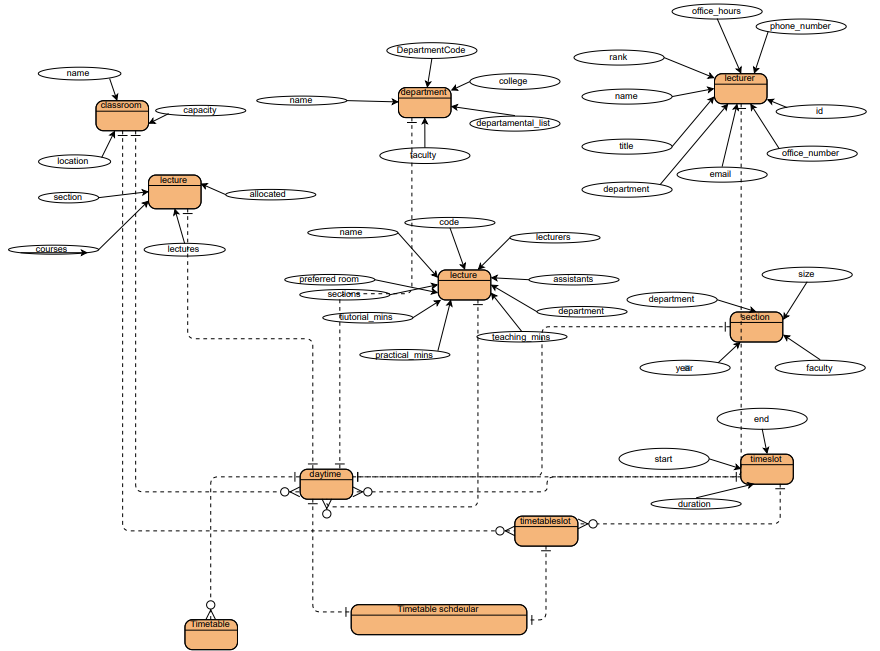
\includegraphics[scale=0.6]{er.png}
ER diagram for the System Database Design
\end{center}

\begin{center}
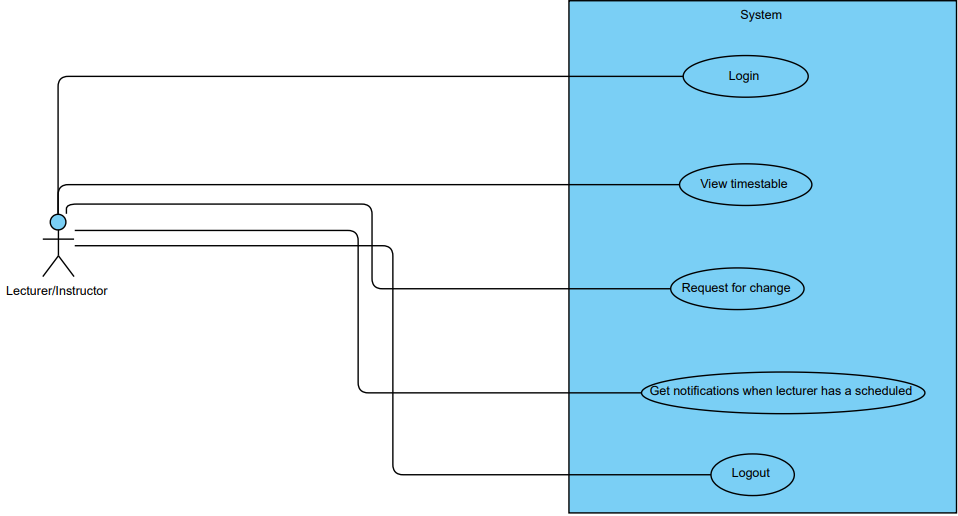
\includegraphics[scale=0.6]{lecturer.png}
Lecturer use case diagram

\end{center}
 Lecturer can log-in to Timetable Management System, using their usernames and
passwords. System displays the main menu if log-in is successful. If the username and
password are not accepted, system displays a message indicating that the username or
password is invalid. Once the lecturer logs in, he or she can perform the processes (use
cases) like view class, view timetable, view master timetable, inquiry class available,
class booking and change password. 
\begin{center}
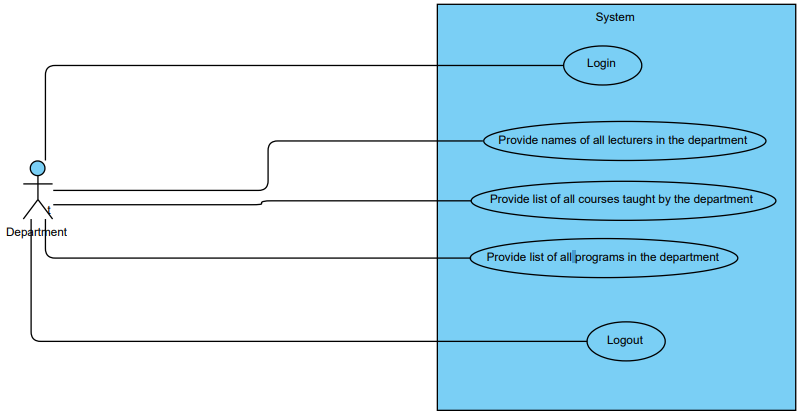
\includegraphics[scale=0.6]{department.png}
Department use case diagram
\end{center}
\begin{center}
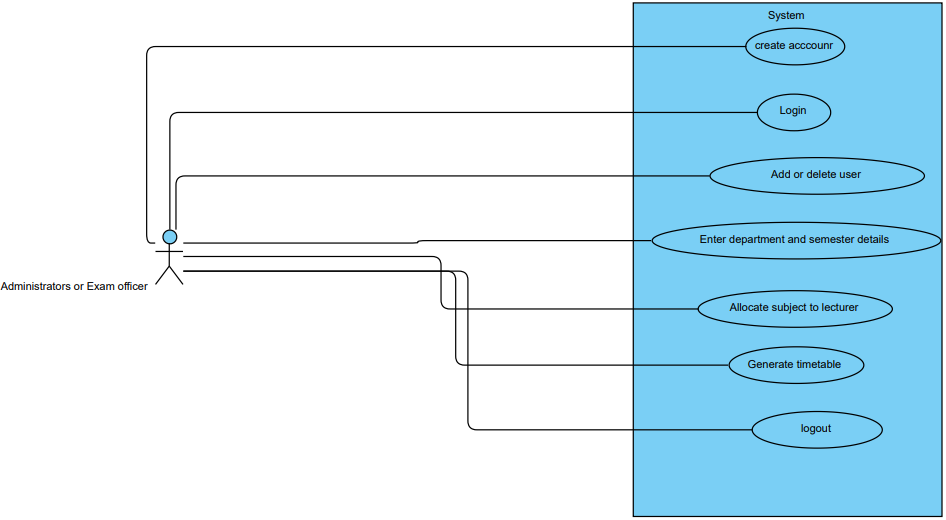
\includegraphics[scale=0.6]{admin.png}
Administrator/Exam officer use case diagram
\end{center}
The administrator does not need to register, as his or her username and password is
fixed in the database. The administrator needs to log in to Timetable Management
System in order to manage the system. Besides logging in, the seven main use cases for
the administrator are student registration, lecturer registration, add class, edit class,
delete class, add courses , edit  and delete course.
 \begin{center}
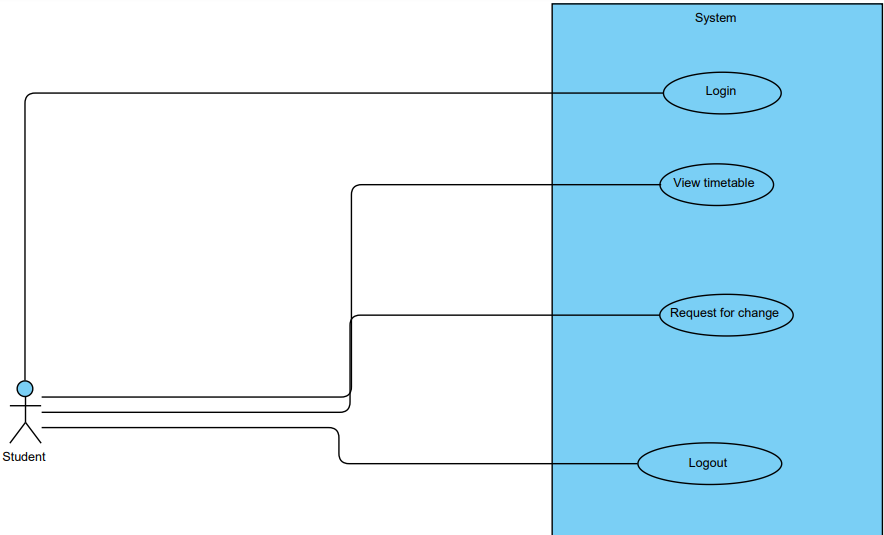
\includegraphics[scale=0.6]{student.png}
Student use case diagram
\end{center}
Student can log-in to Timetable Management System, using their usernames and
passwords. System displays the main menu if log-in is successful. If the username and
password are not accepted, system displays a message indicating that the username or
password is invalid. Once the student logs in, he or she can perform the processes (use
cases) like add subjects, drop subject, view timetable, view registration slip and can
change password

\begin{table}[h!]
  \begin{center}
    \caption{Lecturer use case diagram description.}
    \label{tab:table1}
    \begin{tabular}{|c|c|} 
\hline
      \textbf{Use case} & \textbf{Description} \\
 
      \hline
     Login& It allows the lecture to have access to the system by logging in with a username and password. \\
\hline
      View  &  It allows the lecturer to view his /her lecture schedules on the  timetable.\\
\hline
       Request for change& It allows the lecturer to request for change in lecture times  where necessary\\
\hline
Notification&This facility notifies the lecturer anytime he/she has a lecture.\\
\hline
Logout&  It allows a lecturer to logout of the system.\\
\hline
  \end{tabular}
  \end{center}
\end{table}

\begin{table}[h!]
  \begin{center}
    \caption{ Administrator use case diagram description.}
    \label{tab:table1}
    \begin{tabular}{|c|c|} 
\hline
      \textbf{Use case} & \textbf{Description} \\
 
      \hline
Create Account&This facility allows the administrator to create an admin account for the system\\
\hline
     Login& It allows the administrator must login with username and password generated by the system \\
\hline
      Add/delete  &  It allows the administrator to add or delete  users (i.e lecturers,and students) to have access  to the system.\\
\hline
Enter department and semester details& It allows the admin to enter a department details (Name,courses taught,program streams,lecturers in the department)\\
\hline
Generate timetable& This  feature allows the administrator to generate the timetable if the data requirements are met\\
\hline
       Allocate courses & It allows the administrator to assign lectures for each course.\\
 \hline
Logout&  It allows a administrator to logout of the system.\\
\hline
  \end{tabular}
  \end{center}
\end{table}

\begin{table}[h!]
  \begin{center}
    \caption{ Department use case diagram description.}
    \label{tab:table1}
    \begin{tabular}{|c|c|} 
\hline \textbf{Use case} & \textbf{Description} \\
 \hline
Login &This facility allows the department admin to log into the system\\
\hline
   Provisions of Courses,Programs and Lecturers in department& It allows the department  to add  the list of all courses and lecturers in the department.\\
\hline Logout&  It allows a administrator to logout of the system.\\ \hline
  \end{tabular}
  \end{center}
\end{table}

\begin{table}[h!]
  \begin{center}
    \caption{Student use case diagram description.}
    \label{tab:table1}
    \begin{tabular}{|c|c|} 
\hline
      \textbf{Use case} & \textbf{Description} \\
 
      \hline
     Login& Student cant login with username and password generated by the system \\
\hline
      View& It allows the student to to view  the lectures  timetable \\
\hline
       Request for change& It allows the student to  to request for a change in course schedules\\
\hline
 
Logout&  It allows a student to logout of the system.\\
\hline
  \end{tabular}
  \end{center}
\end{table}
\subsection {Work Flow  modeling}
Activity diagrams are used here to model the flow between the different components.
An activity diagram is needed because the researcher wants to model the workflow of a
use case, and it can show the paths within the use case as well as other use cases. With
activity diagrams, the researcher will be able to illustrate where functionality exists in
the system and how the functionality coordinates with the functionality of other pieces
of the system. The researcher has developed ten activity diagrams for this system. A
brief description will be given to each of the activity diagram in the following pages. 
\begin{center}
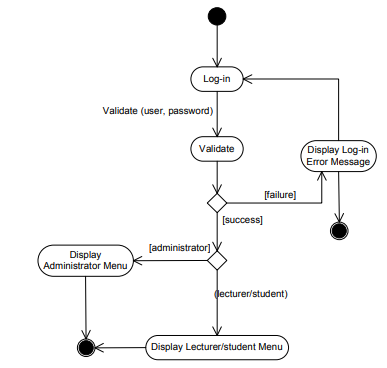
\includegraphics[scale=0.8]{login.png}
Login activity diagram

\end{center}
The figure above shows the activity diagram for Log-in. First, the lecturers, students and
administrator need to log in using the username and password that was created during
registration. The system will validate the username and password. If the password or
username is invalid, an error message will be displayed and the lecturer or student or
administrator can try to log in again. If log in is successful, the system will identify the
user as a lecturer, student or an administrator. If the person logs in as administrator, the
administrator’s menu page will be displayed; else the lecturer or student menu’s page
will be displayed. 
\begin{center}
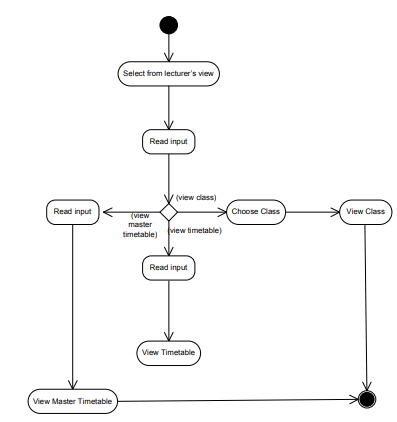
\includegraphics[scale=0.8]{view.png}
Activity diagram for View Class, Timetable or Master Timetable 
\end{center}
The figure above shows the activity diagram for View class, timetable and master
timetable for lecturers. The lecturers can click on the view class or timetable or master
timetable menus and the specific information will be loaded. If the lecturers want to
print their timetable or their master timetable they can click on the button “PRINT”
\subsection{Description and Priority}
$<$Provide a short description of the feature and indicate whether it is of 
High, Medium, or Low priority. You could also include specific priority 
component ratings, such as benefit, penalty, cost, and risk (each rated on
relative scale from a low of 1 to a high of 9).$>$

\subsection{Stimulus/Response Sequences}
$<$List the sequences of user actions and system responses that stimulate the 
behavior defined for this feature. These will correspond to the dialog elements 
associated with use cases.$>$

\subsection{Functional Requirements}
 
\begin{enumerate}
\item Some of the functional requirements of our software product are:
\begin{itemize}
\item Login process/authentication for the administrator,students and lecturers. The administrators can generate the timetable and  make changes when new changes arrive. The lecturers can be authenticated to view their lecture scheduled and request for change in schedules where necessary. The are also notified periodically about their lecture schedule from time to time. The students are also authenticated to have access to their class timetables but they can request for a change when they feel that their class schedules are not favorable.
\item There are 5 Modules for the System
\begin{enumerate}
\item The  Department details 
\item Instructors/Lecturers details
\item The Time Table Allocation details
\item The Courses details
\end{enumerate}
\item Some of the mandatory constraints on the system are:
\begin {enumerate}
\item No two lectures can be taken by the same lecturer except for combined classes.
\item The minimum time for a lecture should be at least one hour and at most four hours.
\item A classroom can be occupied by only one class at a time except  for  combined lectures  where two or more classes can together for a  lecture.
\item A classroom cannot be assigned to a class unless the class size is  less than the capacity of the classroom.
\item There must be no colliding lectures for a particular class. No two lectures should be taken by a class unless they are elective courses where students choose to take one course or the other.
\end {enumerate}
\end {itemize}
\end{enumerate}
 


\chapter{Other Nonfunctional Requirements}

\section{Performance Requirements}

 \begin{itemize}
\item Response time-The system will give responses within 1 second after checking the patient
information and other information.
 \item  User interface- User interface screen will response within 5 seconds.
 \item conformity –The system must conform to the Microsoft accessibility
\end {itemize}
\section{Safety Requirements}
If there is extensive damage to a wide portion of the database due to catastrophic failure, such as a disk crash, the recovery method restores a past copy of the database that was backed up to archival storage (typically tape) and reconstructs a more current state by reapplying or redoing the operations of committed transactions from the backed up log, up to the time of failure.

\section{Security Requirements}
All the administrative and data entry operators have unique logins so system can
understand who is login in to system right now no intruders allowed except system
administrative nobody cannot change record and valuable data.

\section{Software Quality Attributes}
 \begin {itemize}
\item\textbf{Availability} : The system shall be available all the time.
\item \textbf{Correctness}: A bug free software which fulfill the correct need/requirements of the
client
\item \textbf{Maintainability}: The ability to maintain ,modify information and update fix
problems of the system
\item \textbf{ Usability}:  Software can be used again and again without distortion.
\item \textbf{Accessibility}: Administrator and many other users can access the system but the
access level is controlled for each user according to their work scope. 
\item \textbf{Accuracy}:  The reliability on the information/output. Can depend/be sure of the
outcome
\item \textbf{ Stability} : The system outcome/output won’t change time to time. Same output will
be given always for a given input.
\end {itemize}
\section{Business Rules}
\begin{itemize}
 \item Want take the responsibility of failures due to hardware malfunctioning.
\item  Warranty period of maintaining the software would be one year.
\item Additional payments will be analysed and charged for further maintenance
\item  If any error occur due to a user’s improper use. Warranty will not be allocated to it.
\item  No money back returns for the software.
\item Trust bond placement should be done before designing and coding. An advance or an
agreement

\end{itemize}

\chapter{Other Requirements}
 
\section{Appendix A: Glossary}
 No glossary terms available at this time.

\section{Appendix B: Analysis Models}
 \begin{center}
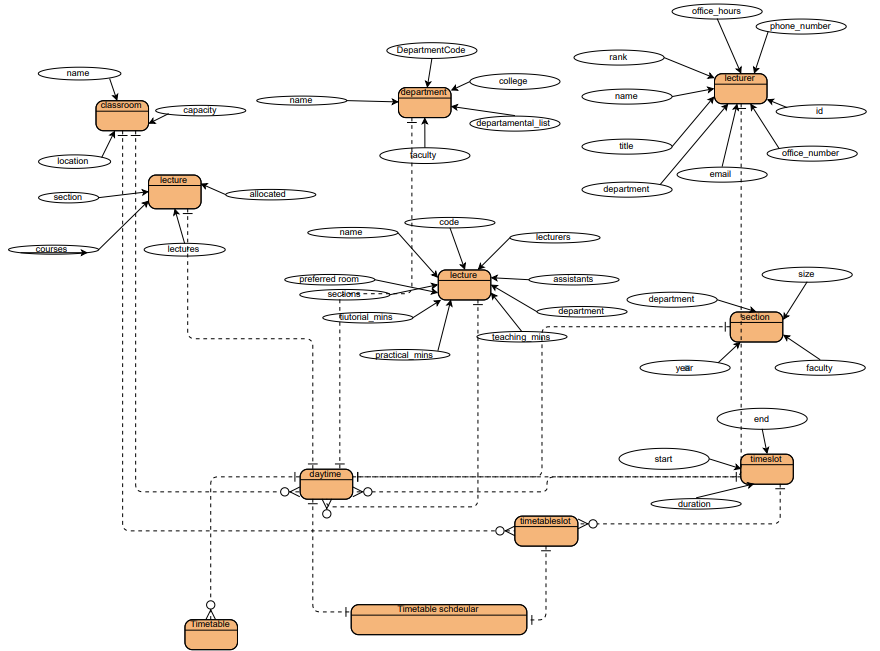
\includegraphics[scale=0.6]{er.png}
\centering
ER diagram for the System Database Design
\end{center}

\begin{center}
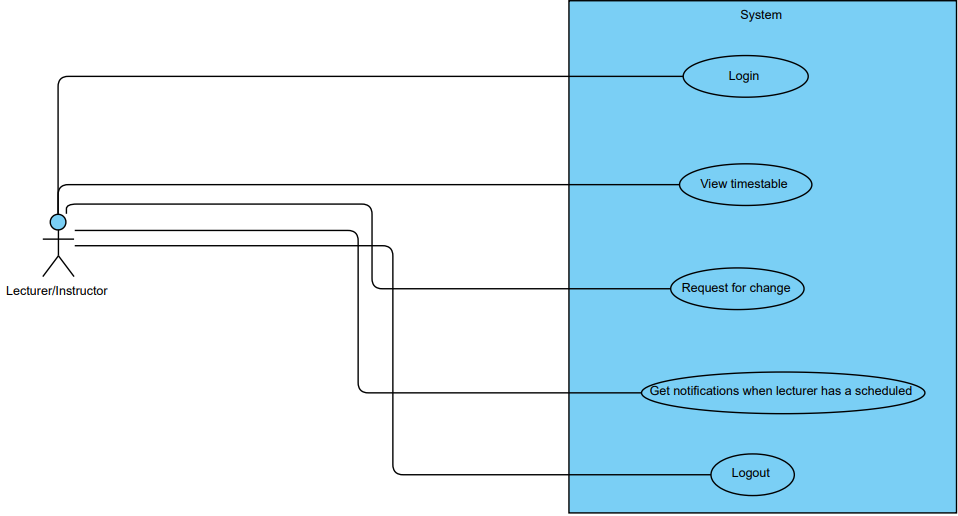
\includegraphics[scale=0.6]{lecturer.png}
Lecturer use case diagram
\end {center}
\begin{center}
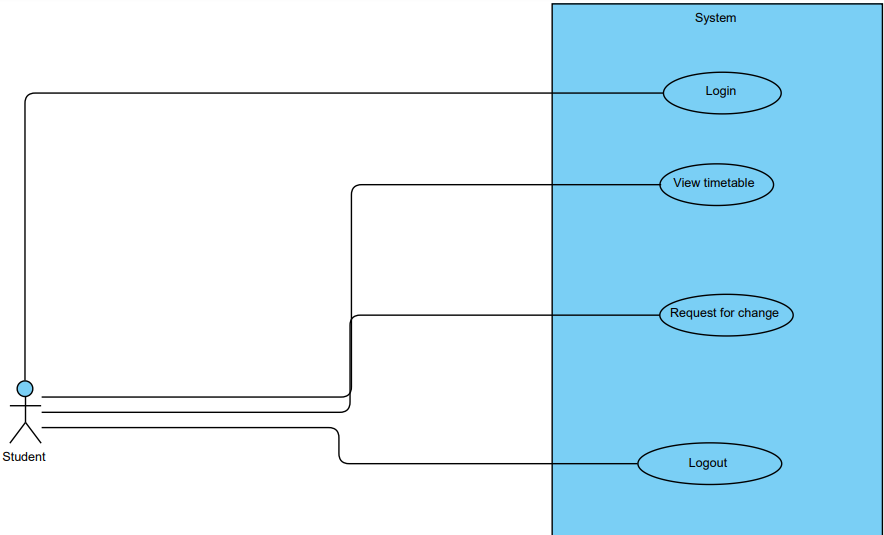
\includegraphics[scale=0.6]{student.png}
Student use case diagram
\end{center}
\begin{center}
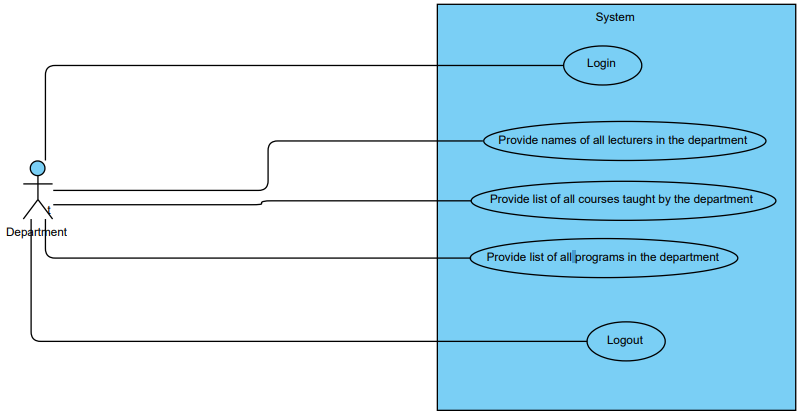
\includegraphics[scale=0.6]{department.png}
Department use case diagram
\end{center}
\begin{center}
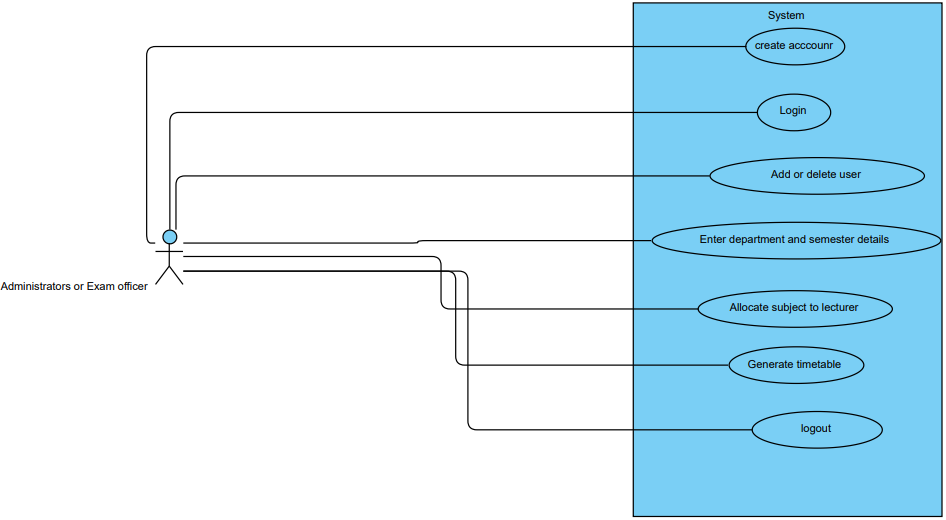
\includegraphics[scale=0.6]{admin.png}
Administrator/Exam officer use case diagram
\end{center}

 
\end{document}
